
%%%%%%%%%%%%%%%%%%%%%%%%%%%%% Define Article %%%%%%%%%%%%%%%%%%%%%%%%%%%%%%%%%%
\documentclass[conference]{IEEEtran}
%%%%%%%%%%%%%%%%%%%%%%%%%%%%%%%%%%%%%%%%%%%%%%%%%%%%%%%%%%%%%%%%%%%%%%%%%%%%%%%

%%%%%%%%%%%%%%%%%%%%%%%%%%%%% Using Packages %%%%%%%%%%%%%%%%%%%%%%%%%%%%%%%%%%
\usepackage{geometry}
\usepackage{graphicx}
\usepackage{amssymb}
\usepackage{amsmath}
\usepackage{amsthm}
    
\usepackage{empheq}
\usepackage{mdframed}
\usepackage{booktabs}
\usepackage{lipsum}
\usepackage{graphicx}
\usepackage{color}
\usepackage{psfrag}
\usepackage{pgfplots}
\usepackage{bm}
\usepackage[spanish]{babel}
\usepackage[utf8]{inputenc} % Codificación UTF-8
\usepackage{amsmath}        % Soporte para ecuaciones matemáticas
\usepackage{graphicx}       % Manejo de imágenes
\usepackage{hyperref}       % Hipervínculos
\usepackage{caption}        % Formato para figuras
\usepackage{multirow}
\usepackage{subcaption}
\usepackage{biblatex}
\usepackage{csquotes}
\usepackage{bookmark}
%%%%%%%%%%%%%%%%%%%%%%%%%%%%%%%%%%%%%%%%%%%%%%%%%%%%%%%%%%%%%%%%%%%%%%%%%%%%%%%

% Other Settings

%%%%%%%%%%%%%%%%%%%%%%%%%% Page Setting %%%%%%%%%%%%%%%%%%%%%%%%%%%%%%%%%%%%%%%
\geometry{a4paper, margin=1in}

%%%%%%%%%%%%%%%%%%%%%%%%%% Define some useful colors %%%%%%%%%%%%%%%%%%%%%%%%%%
\definecolor{ocre}{RGB}{243,102,25}
\definecolor{mygray}{RGB}{243,243,244}
\definecolor{deepGreen}{RGB}{26,111,0}
\definecolor{shallowGreen}{RGB}{235,255,255}
\definecolor{deepBlue}{RGB}{61,124,222}
\definecolor{shallowBlue}{RGB}{235,249,255}
%%%%%%%%%%%%%%%%%%%%%%%%%%%%%%%%%%%%%%%%%%%%%%%%%%%%%%%%%%%%%%%%%%%%%%%%%%%%%%%

%%%%%%%%%%%%%%%%%%%%%%%%%% Define an orangebox command %%%%%%%%%%%%%%%%%%%%%%%%
\newcommand\orangebox[1]{\fcolorbox{ocre}{mygray}{\hspace{1em}#1\hspace{1em}}}
%%%%%%%%%%%%%%%%%%%%%%%%%%%%%%%%%%%%%%%%%%%%%%%%%%%%%%%%%%%%%%%%%%%%%%%%%%%%%%%

%%%%%%%%%%%%%%%%%%%%%%%%%%%% English Environments %%%%%%%%%%%%%%%%%%%%%%%%%%%%%
\newtheoremstyle{mytheoremstyle}{3pt}{3pt}{\normalfont}{0cm}{\rmfamily\bfseries}{}{1em}{{\color{black}\thmname{#1}~\thmnumber{#2}}\thmnote{\,--\,#3}}
\newtheoremstyle{myproblemstyle}{3pt}{3pt}{\normalfont}{0cm}{\rmfamily\bfseries}{}{1em}{{\color{black}\thmname{#1}~\thmnumber{#2}}\thmnote{\,--\,#3}}
\theoremstyle{mytheoremstyle}
\newmdtheoremenv[linewidth=1pt,backgroundcolor=shallowGreen,linecolor=deepGreen,leftmargin=0pt,innerleftmargin=20pt,innerrightmargin=20pt,]{theorem}{Theorem}[section]
\theoremstyle{mytheoremstyle}
\newmdtheoremenv[linewidth=1pt,backgroundcolor=shallowBlue,linecolor=deepBlue,leftmargin=0pt,innerleftmargin=20pt,innerrightmargin=20pt,]{definition}{Definition}[section]
\theoremstyle{myproblemstyle}
\newmdtheoremenv[linecolor=black,leftmargin=0pt,innerleftmargin=10pt,innerrightmargin=10pt,]{problem}{Problem}[section]
%%%%%%%%%%%%%%%%%%%%%%%%%%%%%%%%%%%%%%%%%%%%%%%%%%%%%%%%%%%%%%%%%%%%%%%%%%%%%%%

%%%%%%%%%%%%%%%%%%%%%%%%%%%%%%% Plotting Settings %%%%%%%%%%%%%%%%%%%%%%%%%%%%%
\usepgfplotslibrary{colorbrewer}
\pgfplotsset{width=8cm,compat=1.9}
%%%%%%%%%%%%%%%%%%%%%%%%%%%%%%%%%%%%%%%%%%%%%%%%%%%%%%%%%%%%%%%%%%%%%%%%%%%%%%%

%%%%%%%%%%%%%%%%%%%%%%%%%%%%%%% Title & Author %%%%%%%%%%%%%%%%%%%%%%%%%%%%%%%%
\author{\IEEEauthorblockN{Daniel Fernando Aranda Contreras, Jeremy Carreño Fontalvo,\\ Santiago Silva Quintero}
\IEEEauthorblockA{Escuela E3T, Universidad Industrial de Santander\\
Correo electrónico: \{daniel2221648, jeremy2221647, santiago2231685\}@correo.uis.edu.co}}
%%%%%%%%%%%%%%%%%%%%%%%%%%%%%%%%%%%%%%%%%%%%%%%%%%%%%%%%%%%%%%%%%%%%%%%%%%%%%%%
\begin{document}
% Título
\title{\uppercase{Análisis Termodinámico de un Ciclo Rankine Solar con Tolueno como Fluido de Trabajo y Recuperación de Calor}}
\maketitle
% Resumen
% Palabras clave        
\begin{IEEEkeywords}
    Ciclo Rankine, Energía solar, Tolueno, Recuperación de calor, Turbina de alta presión, Turbina de baja presión, Bomba, Condensador, Calentador, Recalentador, Eficiencia térmica, Generación de entropía, Diagrama T-s.
\end{IEEEkeywords}


\begin{abstract}
    El presente estudio aborda el análisis termodinámico de una planta de energía solar basada en un ciclo Rankine, utilizando la energía solar como fuente de calor primaria. Se emplea tolueno como fluido de trabajo, una elección justificada por la baja temperatura operativa del ciclo en comparación con el agua. El sistema incorpora un calentador, un recalentador, una turbina de alta presión, una turbina de baja presión, un intercambiador de calor recuperativo, una bomba y un condensador. El fluido de transferencia de calor solar ingresa a la planta a $T_{f,in} = 288^{\circ}C$. Se analizan y calculan las presiones en cada estado del ciclo , el trabajo específico de las turbinas y la bomba , la transferencia de calor en los diversos componentes (calentador, recalentador, condensador, intercambiador recuperativo) , y la generación de entropía específica en cada componente principal. Se determina la eficiencia térmica global del ciclo  y se verifica el cumplimiento de la primera y segunda ley de la termodinámica. Adicionalmente, se presenta un diagrama T-s del ciclo  y se investiga la influencia de la presión de recalentamiento sobre la eficiencia de la planta, identificando el intervalo óptimo de esta presión. Finalmente, se analizan los resultados para identificar el equipo con mayor generación de entropía, lo que permite identificar áreas de mejora en el diseño y la operación del ciclo.
\end{abstract}

\section*{ACTIVIDAD}
Ciclo Rankine con fuente solar 

\section*{RESUMEN}
En este informe se analiza el comportamiento de un ciclo Rankine con recalentamiento de una planta de energía solar que emplea tolueno como fluido de trabajo. Se considera la información propuesta que explica cada proceso termodinámico en los componentes del ciclo. Se examinan las tasas de transferencia de calor y de generación de entropía, tomando en cuenta las propiedades termodinámicas del tolueno. Los resultados evidencian beneficios en el uso de este fluido en comparación con el agua, particularmente en sistemas de recuperación de calor a temperaturas intermedias.

\section*{1. Caso de estudio}
Una planta de energía solar consiste en un ciclo Rankine que utiliza la energía solar como fuente de calor. Los receptores parabólicos concentran la energía solar en una tubería que transporta un fluido de transferencia de calor. Este fluido se calienta a medida que fluye a través del campo solar y luego ingresa a la planta de energía. El fluido transfiere calor al fluido de trabajo de la planta de energía para proporcionar la energía térmica que impulsa el ciclo de potencia.

El fluido de transferencia de calor sale del campo y entra a la planta de energía a $T_{f,in} = 288 \,^{\circ}\text{C}$. El fluido ingresa al calentador donde calienta el fluido de trabajo para el ciclo. Debido a que la temperatura de trabajo del ciclo es tan baja, el agua no es un fluido de trabajo muy eficiente; en cambio, se usa tolueno en el ciclo.

El tolueno sale del calentador a:
$T_1 = T_{f,in} - \Delta T_H$
donde $\Delta T_H = 20 \, \text{K}$. El tolueno se expande en la turbina de alta presión desde $P_1 = P_{high} = 1034 \, \text{kPa}$ hasta una presión intermedia $P_2 = P_{reheat} = 250 \, \text{kPa}$ con una eficiencia $\eta_{HPt} = 0.81$.

Luego, el fluido pasa a un recalentador donde se eleva a una nueva temperatura:
$T_3 = T_{f,in} - \Delta T_{RH}$
donde $\Delta T_{RH} = 20 \, \text{K}$. El tolueno que sale de los recalentadores pasa por la turbina de baja presión que tiene una eficiencia de $\eta_{LPt} = 0.78$. La presión de condensación se ajusta de modo que el tolueno que sale del condensador sea líquido saturado a:
$T_6 = T_{amb} + \Delta T_c$
donde $T_{amb} = 35 \,^{\circ}\text{C}$ es la temperatura ambiente y $\Delta T_c = 15 \, \text{K}$. El líquido es bombeado de nuevo a alta presión por una bomba con eficiencia $\eta_p = 0.6$.

Parte del calor del tolueno que sale de la turbina de baja presión se recupera mediante un intercambiador de calor regenerativo, que precalienta el fluido antes de ingresar al calentador. El tolueno entra al condensador a una temperatura dada por:
$T_5 = T_7 - \Delta T_r$
donde $\Delta T_r = 20 \, \text{K}$. Se desprecia la caída de presión a través del calentador, el recalentador, el intercambiador de calor recuperativo y el condensador.

\subsection*{Determinar la presión en cada uno de los estados} 


\begin{table*}[htbp] % El asterisco permite que la tabla ocupe el ancho completo de la página
    \centering
    \caption{Datos termodinámicos de los estados del ciclo}
    \begin{tabular}{|c|c|c|c|c|}
        \hline
        \textbf{Estado} & \textbf{Temperatura (K)} & \textbf{Presión (kPa)} & \textbf{Entalpía (kJ/kg)} & \textbf{Entropía (kJ/kg$\cdot$K)} \\
        \hline
        1 & 541.15 & 1034.00 & 614.74 & 1.298 \\
        2 & 506.54 & 250.00 & 565.05 & 1.321 \\
        3 & 541.15 & 250.00 & 632.51 & 1.450 \\
        4 & 482.81 & 12.29 & 527.03 & 1.513 \\
        5 & 343.15 & 12.29 & 527.03 & 1.513 \\
        6 & 323.15 & 12.29 & -114.68 & -0.324 \\
        7 & 323.15 & 12.29 & -112.65 & -0.318 \\
        8 & 323.15 & 1034.00 & -112.65 & -0.318 \\
        \hline
    \end{tabular}
    \label{tab:datos_termodinamicos}
\end{table*}


Teniendo en cuenta el enunciado, ya tenemos la presión de varios estados en el cuadro \ref{tab:datos_termodinamicos}:
\begin{itemize}
    \item $P_1 = 1034 \, \text{kPa}$ 
    \item $P_2 = 250 \, \text{kPa}$ 
    \item $P_3 = 250 \, \text{kPa}$ 
    \item $P_4 = \text{presión de condensación}$ 
    \item $P_5 = \text{salida del condensador igual a } P_4$ 
    \item $P_6 = \text{se determina con el líquido saturado de } T_6 = 323.15 \, \text{K} \text{ o } 50 \,^{\circ}\text{C} \text{ en las tablas de tolueno.}$ 
    $P_6 = 12.13 \, \text{kPa}$ 
    \item $P_7 = P_6 \text{ es la salida de la bomba.}$ 
    \item $P_8 = P_1 = 1034 \, \text{kPa} \text{ (entrada a la bomba).}$ 
\end{itemize}

\subsection*{El trabajo específico obtenido de la turbina de baja presión $W_{LPt}$, en kJ/kg y la generación de entropía específica en esta turbina $s_{gen,LPt}$, en kJ/kg$\cdot$K.}
El trabajo específico de la turbina a baja presión se calcula como la diferencia entre la entrada y la salida de entalpía:
$W_{LPt} = h_4 - h_3 = 105.483 \, \text{kJ/kg}$ 
La generación de entropía se calcula como la diferencia entre la salida y la entrada de entropía:
$s_{gen} = s_4 - s_3 = 0.06 \, \text{kJ/kg}\cdot\text{K}$ 

\subsection*{El trabajo específico requerido por la bomba $W_P$, en kJ/kg y la generación de entropía específica en la bomba $s_{gen,P}$, en kJ/kg$\cdot$K.}
El trabajo requerido por la bomba nuevamente se calcula como la diferencia de la entrada y la salida de entalpía en la bomba:
$W_P = h_7 - h_6 = 2.030 \, \text{kJ/kg}$ 
La generación específica de entropía en la bomba es la entropía de entrada y salida de esta:
$s_{gen,P} = s_7 - s_6 = 0.006 \, \text{kJ/kg}\cdot\text{K}$ 

\subsection*{La transferencia de calor específica en el intercambiador de calor recuperativo $q_r$, en kJ/kg y la generación de entropía específica $s_{gen,r}$, en kJ/kg$\cdot$K.}
La transferencia de calor específica en el intercambiador de calor recuperativo se calcula como la diferencia de la entrada y salida de las entalpías de los estados en el que se encuentra:
$q_r = h_2 - h_5 = 641.709 \, \text{kJ/kg}$ 
La generación específica de entropía del recuperador se calcula a partir de la irreversibilidad del proceso:
$s_{gen,r} = -1.837 \, \text{kJ/kg}\cdot\text{K}$ 

\subsection*{Trabajo específico y generación de entropía en la turbina de alta presión}
El trabajo específico de la turbina de alta presión se calcula como la diferencia de las entalpías que entran y salen:
$W_{HPt} = h_2 - h_1 = 49.697 \, \text{kJ/kg}$ 
La generación de entropía se calcula como la diferencia de entropía de la generación que entra y sale:
$s_{gen,HPt} = s_2 - s_1 = 0.231 \, \text{kJ/kg}\cdot\text{K}$ 

\subsection*{Transferencia de calor en el calentador, recalentador y condensador}
Para calcular las transferencias de calor específicas en el calentador principal ($q_H$), el recalentador ($q_{RH}$) y el condensador ($q_C$) en un ciclo Rankine regenerativo con recalentamiento, se emplean las diferencias de entalpía entre los estados en los que se lleva a cabo el intercambio térmico.
\begin{align*}
q_H &= h_1 - h_7 = 727.394 \, \text{kJ/kg}  \\
q_{RH} &= h_3 - h_2 = 67.463 \, \text{kJ/kg}  \\
q_C &= q_8 - q_5 = -639.679 \, \text{kJ/kg} 
\end{align*}
La eficiencia térmica de un ciclo de potencia indica la cantidad de energía térmica que realmente se transforma en trabajo útil. Teniendo en cuenta lo anterior, la eficiencia ($\eta$) es:
$\eta = \frac{W_{neto}}{Q_{suministrado}} = \frac{W_{HPt} + W_{LPt} - W_P}{q_H + q_{RH}}$ 
Sustituyendo los valores:
$\eta = \frac{49.697 + 105.483 - 2.030}{727.394 + 67.463}$ 
$\eta = 0.1927$ 
$\eta = 19.27\%$ 

\subsection*{Verifique si el ciclo cumple la primera y la segunda ley de la Termodinámica.} 

\subsubsection*{Primera ley de la termodinámica}
Es conocida como el principio de la conservación de la energía. Establece que:
$(\text{Energía total que entra al sistema}) - (\text{Energía total que sale del sistema}) = (\text{Cambio de energía total del sistema})$ 
$\Delta E_{sistema} = E_{entrada} - E_{salida}$ 
Como se está trabajando en un ciclo cerrado, podemos considerar que $\Delta h_{total} = 0$ y $Q_{neto} = W_{neto}$. Por tanto, tenemos:
$\sum Q_{entra} - \sum Q_{sale} = \sum W_{sale} - \sum W_{entra}$ 

Teniendo en cuenta los estados 1 a 8, y sus respectivas entalpías halladas, tenemos el siguiente análisis, observar cuadro \ref{tab:primera_ley}:
\begin{table*}[htbp] % El asterisco hace que ocupe todo el ancho de la página
    \centering
    \caption{Análisis de la Primera Ley de la Termodinámica}
    \begin{tabular}{|l|l|l|}
    \hline
    \textbf{Proceso} & \textbf{Ecuación} & \textbf{Procedimiento (kJ/kg)} \\
    \hline
    W turbina HP & $W_t = h_1 - h_2$ & $614.74 - 565.05 = 49.69$  \\
    Q recalentamiento & $Q_r = h_3 - h_2$ & $632.51 - 565.05 = 67.46$  \\
    W turbina Lp & $W_{t,lp} = h_3 - h_4$ & $632.51 - 527.03 = 105.48$  \\
    Q total añadido & $Q_{entra} = (h_1 - h_8) + (h_3 - h_2)$ & $727.39 + 67.46 = 794.85$  \\
    W bomba ideal & $W_b = h_8 - h_7$ & $-112.65 - (-112.65) = 0$  \\
    W neto total & $W_{neto} = W_t + W_{t,lp} - W_b$ & $49.69 + 105.48 - 0 = 155.17$  \\
    Q rechazado por condensador & $Q_{salida} = h_5 - h_6$ & $527.03 - (-114.68) = 641.71$  \\
    \hline
    \end{tabular}
    \label{tab:primera_ley}
\end{table*}

Corroboramos que $Q_{neto} = W_{neto}$:
$W_{neto} = W_t + W_{t,lp} - W_b = 49.69 + 105.48 - 0 = 155.17 \, \text{kJ/kg}$ 
$Q_{neto} = Q_{entra} - (h_4 - h_5) - Q_{salida} = 794.85 - 0 - 641.71 = 153.14 \, \text{kJ/kg}$ 
Se puede ver un pequeño margen de error, pero se puede corroborar que $W_{neto} \approx Q_{neto}$.

\subsubsection*{Segunda ley de la termodinámica}
Un proceso debe satisfacer tanto la primera como la segunda ley de la termodinámica para que pueda realizarse. Como es un ciclo cerrado ideal, la entropía debe regresar a su estado inicial, así que se debe cumplir que $\Delta S_{ciclo} = 0$.

Teniendo en cuenta las entropías halladas anteriormente, tenemos (observar cuadro \ref{tab:segunda_ley}):
\begin{table*}[htbp] % El asterisco hace que ocupe todo el ancho de la página
    \centering
    \caption{Análisis de la Segunda Ley de la Termodinámica ($\Delta s$)}
    \begin{tabular}{|l|l|}
    \hline
    \textbf{Proceso} & \textbf{$\Delta s$ (kJ/kg$\cdot$K)} \\
    \hline
    1 y 2 & $\Delta s = 1.321 - 1.298 = 0.023$  \\
    3 y 4 & $\Delta s = 1.513 - 1.450 = 0.063$  \\
    5 y 6 & $\Delta s = -0.324 - 1.513 = -1.837$  \\
    6 y 7 & $\Delta s = -0.318 - (-0.324) = 0.006$  \\
    7 y 8 & $\Delta s = -0.318 - (-0.318) = 0$  \\
    \hline
    \end{tabular}
    \label{tab:segunda_ley}
\end{table*}

\subsection*{Realice el diagrama T-s para el ciclo} 
Teniendo en cuenta los resultados de las tablas dados por los diferentes procesos, se realizó su correspondiente diagrama T-s:
\begin{figure}[ht!]
    \centering
    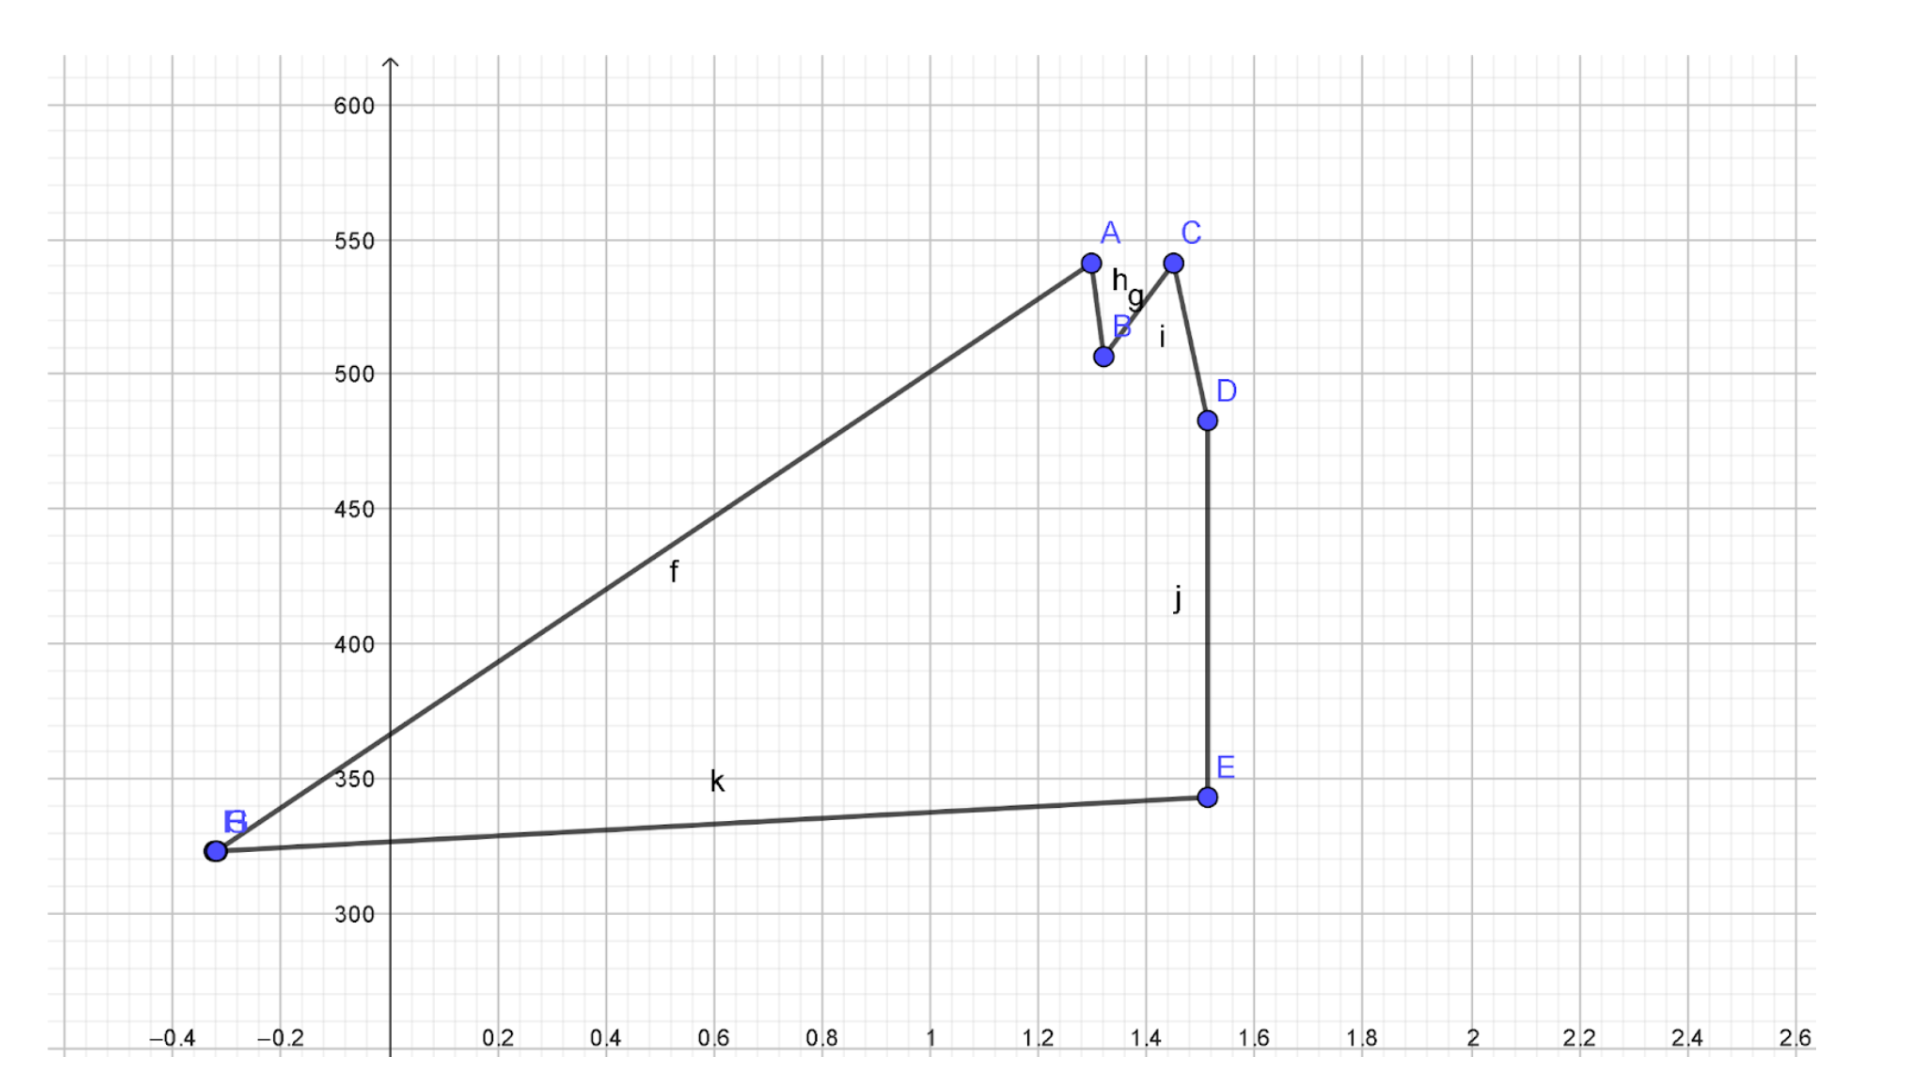
\includegraphics[width=1\textwidth]{Ts_diagram.png} % Asumiendo que guardaste la imagen como Ts_diagram.png
    \caption{Diagrama T-s. Realizado en GeoGebra Clásico \protect\url{https://www.geogebra.org/classic?lang=es}.}
    \label{fig:t-s-diagram}
\end{figure}



% --- Inicio del espacio en blanco ---
\newpage
\clearpage % Asegura que todas las flotantes pendientes se coloquen antes de esta nueva página
\newpage
\clearpage % Genera una segunda página en blanco
% --- Fin del espacio en blanco ---


\section*{CONCLUSIÓN}
Los datos termodinámicos del ciclo Rankine con recalentamiento, presentados en la Tabla \ref{tab:datos_termodinamicos}, evidencian las condiciones de cada estado en términos de temperatura, presión, entalpía y entropía. Estos valores son fundamentales para el análisis energético y exergético del ciclo, permitiendo determinar los trabajos en turbinas y bombas, las transferencias de calor en los intercambiadores y, consecuentemente, la eficiencia térmica global del sistema. La coherencia de estos datos es crucial para verificar el cumplimiento de la primera y segunda ley de la termodinámica, como se detalla en las Tablas \ref{tab:primera_ley} y \ref{tab:segunda_ley}, respectivamente, y para la construcción del diagrama T-s (Figura \ref{fig:t-s-diagram}), que visualiza el comportamiento del ciclo.
\quad

\begin{thebibliography}{1}
    % Nuevas referencias añadidas
    \bibitem{CengelBoles2019}
    Y. A. Çengel, M. A. Boles, and M. Kanoğlu, \emph{Termodinámica}, 9ª ed. México D.F., México: McGraw Hill, 2019.
    \label{CengelBoles2019}

    \bibitem{MoranShapiro2014}
    M. J. Moran, H. N. Shapiro, D. D. Boettner, and M. B. Bailey, \emph{Fundamentals of Engineering Thermodynamics}, 8ª ed. Hoboken, NJ, USA: Wiley, 2014.
    \label{MoranShapiro2014}

\end{thebibliography}

\end{document}  

